\documentclass{beamer}
\beamertemplatenavigationsymbolsempty 

\title{WYSIWYG Stereo Painting}
\author{Dustin Ingram}
\institute{Interactive Computer Graphics, Spring 12-13\\ Drexel University
Department of Computer Science}
\date{\today}

\begin{document}
\maketitle

\begin{frame}
    \frametitle{Introduction}
    \emph{``WYSIWYG Stereo Painting''} by Y.~Kim, H.~Winnem\"{o}ller, and S.~Lee
    (I3D '13 Proceedings of the ACM SIGGRAPH Symposium on Interactive 3D
    Graphics and Games)
    \begin{figure}
        \centering
        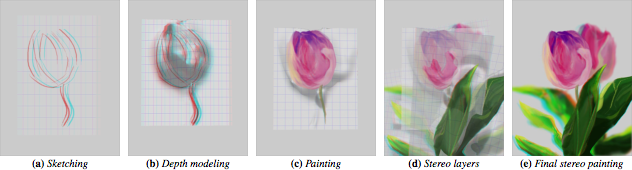
\includegraphics[width=0.8\paperwidth]{f1.png}
    \end{figure}

    What is a stereo image?
    \begin{itemize}
        \item Stereoscopic images and videos give a sense of realistic depth
        perception;
        \item Do so by presenting to slightly different images to each eye.
    \end{itemize}
\end{frame}

\begin{frame}
    \frametitle{Introduction}
    The problem:
    \begin{itemize}
        \item 3D modeling is difficult and time-consuming;
        \item There are no adequate tools are available to-date to create
        artistic (non-photographic) stereo artwork from scratch;
        \item Current paint-on-3D systems were designed to paint on existing
        fixed geometry.
    \end{itemize}
    The goal:
    \begin{itemize}
        \item To answer the question, \emph{``What would a stereo Adobe
        Photoshop or Corel Painter look like?''};
        \item To create a what-you-see-is-what-you-get workflow for stereo
        painting;
        \item To perform essential depth modeling by allowing the artist to
        paint on stereo layers.
    \end{itemize}
\end{frame}

\begin{frame}
    \frametitle{Related Work}
    \begin{itemize}
        \item \textbf{Na\"{i}ve and ad-hoc methods:} hand drawing, requires deep
        understanding of perspective and foreshortening;
        \item \textbf{2.5D approaches:} used for converting monoscopic (regular)
        movies or images to stereoscopic;
        \item \textbf{Paint-in-3D:} user controls a 3D handle, brush strokes are
        painted twice for left and right views;
        \item \textbf{Paint-on-3D (on surface texture):}  user paints onto a 3D
        surface as if through a lens;
        \item \textbf{Paint-on-3D (with surface marks):} incorporates 2D painting
        effects into 3D animation.
    \end{itemize}
\end{frame}

\begin{frame}
    \frametitle{System Design}
    \begin{itemize}
        \item Follows the common paint-on-3D approach;
        \item Adds the concept of \emph{stereo layers}:
        \begin{itemize}
            \item A generalization of the traditional layer in monoscopic image
            editing tools;
            \item A concept that is well known to artists, thus lowering the
            learning curve.
        \end{itemize}
        \item Key differences between a paint-on-3D approach:
        \begin{itemize}
            \item Postponable modeling - does not require complex 3D models;
            \item Fa\c{c}ade modeling - does not require modeling the entire 3D
            geometry;
            \item Painted contours - removes the correlation between object
            geometry and object paint;
            \item Perception-based modeling - ability to add other depth cues,
            such as shading.
        \end{itemize}
    \end{itemize}
\end{frame}

\begin{frame}
    \frametitle{Stereo Paint Brush}
    \begin{itemize}
        \item The system converts 2D user input into 3D stroke paths;
        \item This produces two corresponding paths for the left and right
        views;
        \item These paths are rendered by mapping ``splats'' along the path
        according to brush attributes;
        \item Stroke similarity is maintained between views by evaluating an
        optimization function that considers both.
    \end{itemize}
\end{frame}

\begin{frame}
    \frametitle{Stereo Depth Brush}
    \begin{itemize}
        \item This tool allows for the manipulation the depth buffers on the
        stereo layer;
        \item Provides a number of manipulations, including displace, move,
        magnify, pinch, and blob;
        \item Each of these actions changes the underlying 3D geometry in
        Euclidean space;
        \item These manipulations are unique foe each fixed viewpoint, as they
        cannot be directly mapped onto another viewpoint;
        \item Two main brush interactions are provided:
        \begin{itemize}
            \item Displacement brush - places positive or negative values onto
            the stereo layer to deform the mesh grid;
            \item Smoothing brush - for de-emphasizing or removing extrusions.
        \end{itemize}
    \end{itemize}
\end{frame}

\begin{frame}
    \frametitle{Multiple Stereo Layers}
    \begin{itemize}
        \item A single layer only offers similar functionality to existing 2.5D
        approaches;
        \item Combining multiple layers allows for complex depth and layering
        effects;
        \item Some additional features multiple layers adds:
        \begin{itemize}
            \item Duplication - essentially copying and cloning of layers;
            \item Merge - useful for modeling a more complicated geometry;
            \item Copy \& paste - projection of brush strokes onto another
            layer;
        \end{itemize}
    \end{itemize}
\end{frame}

\begin{frame}
    \frametitle{Experimental Results}
    \begin{itemize}
        \item A number of artists have used the system prior to the publication
        of the paper;
        \item The visual looks are very distinct, indicating that the system is
        versatile and allows an artist to achieve a unique, personal style;
        \item Some feedback from artists who have used the system:
        \begin{itemize}
            \item Most artists had experience with digital tools and 3D modeling
            systems;
            \item Multiple workflows were developed in the course of each artist
            using the tools;
            \item The time to paint the first painting was high, with a greatly
            reduced time to paint subsequent images;
            \item Artists expressed that the system was ``fun'' and were excited
            about this new art form.
        \end{itemize}
    \end{itemize}
\end{frame}

\begin{frame}
    \frametitle{Conclusion}
    \begin{itemize}
        \item The stereo painting system realizes a holistic solution for
        from-scratch WYSIWYG stereo painting;
        \item The system requires and supports modeling only essential depth for
        a stereo painting;
        \item The response from artists was positive in nature.
    \end{itemize}
\end{frame}

\end{document}
